\ifdefined \buildingFullOPALManual \else


%\ifx \@buildingFullOPALManual \@empty
%\else

%\documentclass[12pt,a4paper]{report}
\documentclass[a4paper]{book}

%% does not work in Latex2Html mode
%\usepackage{hyperref}

\usepackage[T1]{fontenc}
\usepackage{url}
\usepackage{html}
\usepackage{epic}
\usepackage{eepic}
\usepackage{makeidx}
\usepackage{array}
\usepackage{times}
\usepackage{amsmath}
\usepackage{amsxtra}
\usepackage{bm}
\usepackage[thin,thinp,thinc]{esdiff}
\usepackage{graphicx}
\usepackage{dingbat}
\usepackage{color}
\usepackage{subfig}
\usepackage{boxedminipage}
\usepackage{alltt}
\usepackage{nicefrac}
\usepackage{calc}
%\usepackage{pdfdraftcopy}             % Draft
\usepackage{tikz}
\usetikzlibrary{
  er,3d,calc,fadings,trees,positioning,arrows,chains,decorations.pathreplacing,
  decorations.pathmorphing,shapes,shapes.symbols,shapes.arrows,matrix,through,decorations.text
}

\tikzset{
  >=stealth',
  punktchain/.style={rectangle,rounded corners, draw=black, very thick,text width=10em,
                     minimum height=3em, text centered, on chain},
  line/.style={draw, thick, <-},
  element/.style={tape,top color=white,bottom color=blue!50!black!60!,minimum width=8em,
                  draw=blue!40!black!90, very thick,text width=10em, minimum height=3.5em,
                  text centered, on chain},
  every join/.style={->, thick,shorten >=1pt},
  tuborg/.style={decorate},
  tubnode/.style={midway, right=2pt}
}

\tikzstyle{material}=[draw, fill=blue!20, text width=16.0em, text centered, minimum height=1.5em]
\tikzstyle{diagramstep} = [material, text width=20em, minimum width=10em, minimum height=3em, rounded corners]
\tikzstyle{line} = [draw, thick, color=black!50, -latex']

\usepackage{booktabs}
\usepackage{xspace}
\usepackage{xstring}

\usepackage{fancyvrb}
\usepackage{rotating}
\usepackage{float}

\usepackage{tabularx}
\usepackage{longtable}
\setcounter{LTchunksize}{3}

\usepackage[section]{placeins}
\usepackage{MnSymbol}
\usepackage{microtype}
\usepackage{setspace}
\usepackage{dcolumn}

\usepackage[vmargin={3.0cm,3.0cm},
            hmargin={2.0cm,3.0cm}]{geometry}

\usepackage{upgreek}
\usepackage[binary-units=true]{siunitx}
\sisetup{exponent-product = \cdot,math-ohm=\Upomega,text-ohm=\ensuremath{\Upomega}}
\DeclareSIUnit{\clight}{c}
\DeclareSIUnit\gauss{Ga}

\usepackage{engord}
\usepackage{wasysym}
\DeclareSIUnit[number-unit-product = \,]{\permill}{\permil}

\usepackage{hyperref}
\hypersetup{
    pdftitle          = The OPAL Framework,
    pdfauthor         = {Andreas Adelmann, Achim Gsell, Valeria Rizzoglio, Christof Metzger-Kraus,
                         Yves Ineichen, Xiaoying Pang, Steve Russell, Chuan Wang, Jianjun Yang,
                         Suzanne Sheehy, Chris Rogers, Daniel Winklehner},
    pdfsubject        = User's Reference Manual,
    pdffitwindow      = true,               % page fit to window when opened
    pdfnewwindow      = true,               % links in new window
    colorlinks        = true,               % false: boxed links; true: colored links
    linkcolor         = black!80!green,     % color of internal links
    citecolor         = black!20!red,       % color of links to bibliography
    urlcolor          = blue,               % color of external links
    breaklinks        = true,
    bookmarksnumbered = true,
    plainpages        = false
}

\usepackage{ifthen}

\newif \iflinuxwindows
\linuxwindowstrue   % set this to true when building the manual on Linux or Windows
\iflinuxwindows
\usepackage{epstopdf}
\fi

\usepackage[backend=biber,
            style=phys,
            biblabel=brackets,
            maxnames=3,
            doi=true,
            isbn=true,
            url=true]{biblatex}
%---- macros ----

\renewcommand{\topfraction}{1.0}
\renewcommand{\bottomfraction}{1.0}
\renewcommand{\textfraction}{0.0}
\renewcommand{\arraystretch}{2.0}
\newenvironment{tex2html_nowrap}{}{}


\newcommand{\Newline}{\hfil \\}


\newsavebox{\ExampleBox}
\newenvironment{example}
 {\VerbatimEnvironment
  \begin{flushleft}
  \begin{lrbox}{\ExampleBox}
    \begin{minipage}{\linewidth}
  \begin{Verbatim}[frame=lines,xleftmargin=0cm,fontsize=\footnotesize,samepage=true]}
 {\end{Verbatim}
  \end{minipage}
  \end{lrbox}
  \mbox{\usebox{\ExampleBox}}
  \end{flushleft}
 }

\newenvironment{longexample}
{\Verbatim[frame=lines,xleftmargin=0mm,fontsize=\footnotesize]}
{\endVerbatim}

%\examplefromfile{filename} reads in a text file and displays it in the document.
\newcommand{\examplefromfile}[1]{
\VerbatimInput[frame=lines,xleftmargin=0mm,fontsize=\footnotesize,label=\texttt{#1}]{#1}}

%for upright d of differentials
\makeatletter
\newcount\my@repeat@count

\newcommand{\myrepeat}[2]{%
  \begingroup
  \my@repeat@count=\z@
  \@whilenum\my@repeat@count<#1\do{#2\advance\my@repeat@count\@ne}%
  \endgroup
}

\newcommand{\differential}[1]{\ifstrempty{#1}{\ES@dop\ES@difint}{\ES@dop^{#1}\ES@difint}}
\newcommand{\pdifferential}[1]{\ifstrempty{#1}{{\partial\,}}{{\partial^{#1}\,}}}

\makeatother

\newcommand{\der}[3][]{\frac{\differential{#1}#2}{\differential{}\ifstrempty{#1}{#3}{#3^#1}}}
\newcommand{\parder}[3][]{\frac{\pdifferential{#1}#2}{\pdifferential{}\ifstrempty{#1}{#3}{#3^#1}}}
\newcommand{\niceder}[3][]{\nicefrac{\differential{#1}#2}{\differential{}\ifstrempty{#1}{#3}{#3^#1}}}
\newcommand{\uglyder}[3][]{{\differential{#1}#2}/{\differential{}\ifstrempty{#1}{#3}{#3^#1}}}
\newcommand{\uglyparder}[3][]{{\pdifferential{#1}#2}/{\pdifferential{}\ifstrempty{#1}{#3}{#3^#1}}}
\newcommand{\dd}[1][]{\; \differential{#1}}
\newcommand{\primed}{^{\prime}}
\newcommand{\dprimed}{^{\prime\prime}}
\newcommand{\nprimed}[1]{^{\myrepeat{#1}{\prime}}}

%Editing Macros
\newcommand{\TODO}[1]{{\color{red}\ifthenelse{\boolean{ShowDebug}}{[TODO: #1]}{}}}



%text in gray box
\newsavebox{\fmbox}
\definecolor{lightgray}{gray}{0.95}
\newenvironment{fmpage}
   {\vspace{-1.0cm}\begin{lrbox}{\fmbox}\begin{minipage}[t]{13.5cm}\vspace{0.1cm}}
   {\vspace{-0.4cm}\end{minipage}\end{lrbox}\begin{center}\fcolorbox{black}{lightgray}{\usebox{\fmbox}}\end{center}}


% Definition new signes
\newcommand{\R}{{\mathbb R}} % real numbers
\newcommand{\Q}{{\mathbb Q}} % rational numbers
\newcommand{\Z}{{\mathbb Z}} % integer numbers
\newcommand{\N}{{\mathbb N}} % natural numbers

\newcommand{\mad}{\textsc{mad}\xspace}
\newcommand{\madnine}{\textsc{mad9}\xspace}
\newcommand{\madninep}{\textsc{mad9p}\xspace}
\newcommand{\madeight}{\textsc{mad8}\xspace}
\newcommand{\classic}{\textsc{classic}\xspace}

\makeatletter
\newcommand{\opal@impl}{\textsc{Opal}}
\newcommand{\opalt@impl}{\textsc{Opal-t}}
\newcommand{\opalcycl@impl}{\textsc{Opal-cycl}}
\newcommand{\opalmap@impl}{\textsc{Opal-map}}
\newcommand{\opalenv@impl}{\textsc{Opal-e}}

\newcommand{\opal}{\opal@impl\xspace}
\newcommand{\opalt}{\opalt@impl\xspace}
\newcommand{\opalcycl}{\opalcycl@impl\xspace}
\newcommand{\opalmap}{\opalmap@impl\xspace}
\newcommand{\opalenv}{\opalenv@impl\xspace}

\newcommand{\noopalt}{\leftthumbsdown \opalt@impl\xspace}
\newcommand{\noopalcycl}{\leftthumbsdown \opalcycl@impl\xspace}
\newcommand{\noopalmap}{\leftthumbsdown \opalmap@impl\xspace}
\newcommand{\noopalenv}{\leftthumbsdown \opalenv@impl\xspace}
\makeatother

\newcommand{\impactt}{\textsc{Impact-t}\xspace}
\newcommand{\partroot}{\textsc{H5root}}


\newcommand{\latermore}{More details will be given in Version 1.6.0}


\newcommand{\lieop}[1]{{:}{#1}{:}}

\newcommand{\rms}[1]{\overset{\sim}{#1}}

\newcommand{\sprod}{\cdot}
\newcommand{\vprod}{\times}
\newcommand{\matr}[1]{\mathcal{#1}}
\renewcommand{\vec}[1]{{\bm{#1}}}
\newcommand{\transpose}[1]{#1^\intercal}
\renewcommand{\epsilon}{\varepsilon}

\newcommand{\keyword}[2][]{\ifstrempty{#1}{\texttt{\expandafter\MakeUppercase\expandafter{#2}}}{\hyperref[#1]{\texttt{\expandafter\MakeUppercase\expandafter{#2}}}}}
\newcommand{\tabline}[3][]{\keyword[#1]{#2}& #3 \\}
\newcommand{\tabheadcell}[1]{{\bfseries #1}}

\newcommand*\kdescriptionlabel[1]{\hspace\labelsep
                                \normalfont\keyword{#1}\index{#1}}
\makeatletter
\newenvironment{kdescription}
               {\list{}{\labelwidth\z@ \itemindent-\leftmargin
                        \let\makelabel\kdescriptionlabel}}
               {\endlist}
\makeatother

\ExplSyntaxOn
\NewDocumentCommand{\tabhead}{ m }
 {
  \seq_set_split:Nnn \l_tmpa_seq { & } { #1 }
  \bfseries \seq_use:Nn \l_tmpa_seq { & \bfseries } \\
 }

\NewDocumentCommand \multrefImpl { O{ } m m m } {
  \ifnumgreater{\clist_count:n {#4}}{1}{
    \seq_set_from_clist:Nn \l_tmpa_seq { #4 }

    \seq_set_map:NNn \l_tmpb_seq \l_tmpa_seq { \exp_not:n { \ref{#3:##1} } }
    \ifstrempty{#1}{#2s}{#1}~\seq_use:Nnnn \l_tmpb_seq {\ and\ } {,\ } {,\ and\ }
  }{
    #2~\ref{#3:#4}
  }
}

\NewDocumentCommand \multeqnrefImpl { m } {
  \ifnumgreater{\clist_count:n {#1}}{1}{
    \seq_set_from_clist:Nn \l_tmpa_seq { #1 }

    \seq_set_map:NNn \l_tmpb_seq \l_tmpa_seq { \exp_not:n { \eqref{eq:##1} } }
    Equations~\seq_use:Nnnn \l_tmpb_seq {\ and\ } {,\ } {,\ and\ }
  }{
    Equation~\eqref{eq:#1}
  }
}
\ExplSyntaxOff


%Abbreviations for Equations, Figures, and Tables
%\newcommand{\Equation}[1]{Equation~\eqref{#1}}

\newcommand{\bibref}[2]{#1 \cite{bib:#2}}
\newcommand{\figref}[1]{\multrefImpl{Figure}{fig}{#1}}
\newcommand{\chpref}[1]{\multrefImpl{Chapter}{chp}{#1}}
\newcommand{\appref}[1]{\multrefImpl[Appendices]{Appendix}{chp}{#1}}
\newcommand{\secref}[1]{\multrefImpl{Section}{sec}{#1}}
\newcommand{\ssecref}[1]{\multrefImpl{Section}{ssec}{#1}}
\newcommand{\tabref}[1]{\multrefImpl{Table}{tab}{#1}}
\newcommand{\eqnref}[1]{\multeqnrefImpl{#1}}

\newcommand{\seefig}[1]{(see~\figref{#1})}
\newcommand{\seechp}[1]{(see~\chpref{#1})}
\newcommand{\seesec}[1]{(see~\secref{#1})}
\newcommand{\seessec}[1]{(see~\ssecref{#1})}
\newcommand{\seetab}[1]{(see~\tabref{#1})}
\newcommand{\seeeqn}[1]{(see~\eqnref{#1})}

\newcommand{\filename}[1]{\emph{#1}}


% Define distances for bordering
\newcommand{\blockdist}{1.3}
\newcommand{\edgedist}{1.5}
\newcommand{\diagramstep}[2]{node (p#1) [diagramstep] {#2}}


% place chapter title page on odd pages
\let\stdchapter\chapter
\makeatletter
\renewcommand*{\chapter}{\if@openright\cleardoublepage\else\clearpage\fi\stdchapter}

\makeatother

\IfFileExists{./version.tex}{%
  \newcommand{\opalversion}[1]{Version \ifstrempty{#1}{1.9.0}{#1}\xspace}
%
}%
{%
  \newcommand{\opalversion}[1]{\ifstrempty{#1}{current Version}{Version #1}\xspace}%
}
\newboolean{ShowMap}
\setboolean{ShowMap}{false}

\newboolean{ShowEnv}
\setboolean{ShowEnv}{false}

\newboolean{ShowDebug}
\setboolean{ShowDebug}{false}

%----Control Structures
\newboolean{FullOPALManual}
\setboolean{FullOPALManual}{false}


\makeindex


\bibliography{bibliography}
\begin{document}

\fi

\chapter{\opalcycl}
\label{chp:opalcycl}
\index{OPAL-cycl}


% -- -- -- -- -- -- Section -- -- -- -- -- --
\section{Introduction}

\opalcycl, as one of the flavors of the \opal framework,  is a fully three-dimensional parallel beam dynamics simulation program dedicated to future high intensity cyclotrons and FFAG. it tracks multiple particles  which takes into account the space charge effects. For the first time in the cyclotron community, \opalcycl has the capability of tracking multiple bunches simultaneously
and take into account the beam-beam effects of the radially neighboring bunches (we call it neighboring bunch effects for short)
by using a self-consistent numerical simulation model.

Apart from the multi-particle simulation mode, \opalcycl also has two other serial tracking modes for conventional cyclotron machine design. One mode is the single particle tracking mode, which is a useful tool for the preliminary design of a new cyclotron.  It allows one to compute basic parameters, such as reference orbit, phase shift history, stable region, and matching phase ellipse. The other one is the tune calculation mode, which can be used to compute the betatron oscillation frequency.
This is useful for evaluating the focusing characteristics of a given magnetic field map.

In addition, the widely used plugin elements, including collimator, radial profile probe, septum, trim-coil field and charge stripper,  are currently implemented in \opalcycl. These functionalities are very useful for designing, commissioning and upgrading of cyclotrons and FFAGs.

\section{Tracking modes}
According to the number of particles defined by the argument \keyword{npart} in \keyword{beam} \seechp{beam} ,
\opalcycl  works in one of the following three operation modes automatically.


\subsection{Single Particle Tracking mode}

  In this mode, only one particle is tracked, either with acceleration or not.  Working in this mode, \opalcycl
  can be used as a tool during the preliminary design phase of a cyclotron.

  The 6D parameters of a single particle in the initial local frame must be read from a file. To do this, in the \opal input file,
  the command line \keyword{DISTRIBUTION} \seechp{distribution} should be defined like this:
\begin{example}
  Dist1: DISTRIBUTION, TYPE=fromfile, FNAME="PartDatabase.dat";
\end{example}
 where the file \filename{PartDatabase.dat} should have two lines:
\begin{example}
 1
 0.001 0.001   0.001   0.001   0.001  0.001
\end{example}
The number in the first line is the total number of particles.
In the second line the data represents $x, p_x, y,$$ p_y, z, p_z$ in the local reference frame. Their units are described in \secref{variablesopalcycl}.

Please don't try to run this mode in parallel environment. You should believe that a single processor of the \engordnumber{21} century is capable of doing
the single particle tracking.

\subsection{Tune Calculation mode}

  In this mode, two particles are tracked, one with all data is set to zero is the reference particle and another one is an off-centering particle
  which is off-centered in both $r$ and $z$ directions. Working in this mode, \opalcycl can calculate the betatron oscillation frequency $\nu_r$ and $\nu_z$ for different energies to evaluate the focusing characteristics
  for a given magnetic field.

  Like the single particle tracking mode,
  the initial 6D parameters of the two particles in the local reference frame must be read from a file, too.
  In the file should has three lines:
\begin{example}
 2
 0.0   0.0   0.0   0.0   0.0   0.0
 0.001 0.0   0.0   0.0   0.001  0.0
\end{example}

When the total particle number equals 2, this mode is triggered automatically.
Only the element \keyword{CYCLOTRON} in the beam line is used and other elements are omitted if any exists.

Please don't try to run this mode in parallel environment, either.


\subsection{Multi-particle tracking mode}

  In this mode, large scale particles can be tracked simultaneously, either with space charge or not,
  either single bunch or multi-bunch, either serial or parallel environment,
  either reading the initial distribution from a file or generating a typical distribution,
  either running from the beginning or restarting from the last step of a former simulation.

  Because this is the main mode as well as the key part of \opalcycl,
  we will describe this in detail in \secref{opalcycl:MultiBunch}.




% -- -- -- -- -- -- Section -- -- -- -- -- --
\section{Variables in \opalcycl}
\label{sec:variablesopalcycl}
\index{OPAL-cycl:Variables}

\label{sec:opalcycl:canon}
\index{Canonical Variables}
\index{Variables!Canonical}

\opalcycl uses the following canonical variables to describe the motion of particles:

\begin{description}
\item[X]
  Horizontal position $x$ of a particle in given global Cartesian coordinates [\si{\meter}].

\item[PX]
  Horizontal canonical momentum [\si{\electronvolt/\clight}].

\item[Y]
  Longitudinal position $y$ of a particle in global Cartesian coordinates [\si{\meter}].

\item[PY]
  Longitudinal canonical momentum [\si{\electronvolt/\clight}].

\item[Z]
  Vertical position $z$ of a particle in global Cartesian coordinates [\si{\meter}].

\item[PZ]
  Vertical canonical momentum [\si{\electronvolt/\clight}].

\end{description}

The independent variable is: \textbf{t} [\si{\second}].


\subsubsection{NOTE: unit conversion of momentum in \opalt and \opalcycl}
Convert $\beta_x \gamma$ [dimensionless] to [\si{\milli\radian}],

\begin{equation}
\label{eq:betagamma1}
(\beta\gamma)_{\text{ref}}=\frac{P}{m_0c}=\frac{Pc}{m_0c^2},
\end{equation}
\begin{equation}
\label{eq:betagamma2}
P_x[\si{\milli\radian}]=1000\times\frac{(\beta_x\gamma)}{(\beta\gamma)_{\text{ref}}}.
\end{equation}

Convert from [\si{\electronvolt/\clight}] to $\beta_x\gamma$ [dimensionless],
\begin{equation}
\label{eq:eVtobetagamma}
(\beta_x\gamma)=\sqrt{(\frac{P_x[\si{\electronvolt/\clight}]}{m_0c}+1)^2-1}.
\end{equation}

This may be deduced by analogy for the $y$ and $z$ directions.

\subsection{The initial distribution in the local reference frame }
\label{sec:opalcycl:localframe}
The initial distribution of the bunch,
either read from file or generated by a distribution generator \seechp{distribution},
is specified in the local reference frame of the \opalcycl Cartesian coordinate system \seesec{opalcycl:canon}.
At the beginning of the run, the 6 phase space variables \((x, y, z, p_x, p_y, p_z)\)
are transformed to the global Cartesian coordinates using the starting coordinates $r_0$ (\keyword{RINIT}), $\phi_0$ (\keyword{PHIINIT}), and $z_0$ (\keyword{ZINIT}),
and the starting momenta $p_{r0}$ (\keyword{PRINIT}), and $p_{z0}$ (\keyword{PZINIT}) of the reference particle, defined
in the \keyword{CYCLOTRON} element \seesec{cyclotron}. Note that $p_{\phi 0}$ is calculated
automatically from $p_{total}$, $p_{r0}$, and $p_{z0}$.

\begin{align*}
X &= x\cos(\phi_0) - y\sin(\phi_0) + r_0\cos(\phi_0)  \\
Y &= x\sin(\phi_0) + y\cos(\phi_0) + r_0\sin(\phi_0)  \\
Z &= z + z_0
\end{align*}
\begin{align*}
PX &= (p_x+p_{r0})\cos(\phi_0) - (p_y+p_{\phi 0})\sin(\phi_0) \\
PY &= (p_x+p_{r0})\sin(\phi_0) + (p_y+p_{\phi 0})\cos(\phi_0) \\
PZ &= p_z + p_{z0}
\end{align*}


% -- -- -- -- -- -- Section -- -- -- -- -- --
\section{Field Maps}
\label{sec:opalcycl:fieldmap}
In \opalcycl, the magnetic field on the median plane is read from an ASCII type file. The field data should be stored in the cylinder coordinates frame (because the field map on the median plane of the cyclotron is usually measured in this frame).

There are two possible situations. One is the real field map on median plane of the exist cyclotron machine using measurement equipment.
Limited by the narrow gaps of magnets, in most cases with cyclotrons, only vertical field $B_z$ on the median plane ($z=0$) is measured.
Since the magnetic field data off the median plane field components is necessary for those particles with $z \neq 0$, the field need to be expanded in $Z$ direction.
According to the approach given by Gordon and Taivassalo, by using a magnetic potential and measured $B_z$ on the median plane,
at the point $(r,\theta, z)$ in cylindrical polar coordinates, the \engordnumber{3} order field can be written as
\begin{eqnarray}\label{eq:Bfield}
  B_r(r,\theta, z) & = & z\diffp{B_z}{ r}-\frac{1}{6}z^3 C_r, \nonumber\\
  B_\theta(r,\theta, z) & = & \frac{z}{r}\diffp{B_z}{\theta}-\frac{1}{6}\frac{z^3}{r} C_{\theta}, \\
  B_z(r,\theta, z) & = & B_z-\frac{1}{2}z^2 C_z,  \nonumber
\end{eqnarray}
where $B_z\equiv B_z(r, \theta, 0)$ and
\begin{eqnarray}\label{eq:Bcoeff}
  C_r & = & \diffp[3]{B_z}{r} + \frac{1}{r}\diffp[2]{B_z}{r} - \frac{1}{r^2}\diffp{B_z}{r}
        + \frac{1}{r^2}\diffp{B_z}{{r}{\theta^2}} - 2\frac{1}{r^3}\diffp[2]{B_z}{\theta}, \nonumber  \\
  C_{\theta} & = & \frac{1}{r}\diffp{B_z}{{r}{\theta}} + \diffp{B_z}{{r^2}{\theta}}
        + \frac{1}{r^2}\diffp[3]{B_z}{\theta},  \\
  C_z & = & \frac{1}{r}\diffp{B_z}{r} + \diffp[2]{B_z}{r} + \frac{1}{r^2}\diffp[2]{B_z}{\theta}. \nonumber
\end{eqnarray}

All the partial differential coefficients are on the median plane and can be calculated by interpolation. \opalcycl uses  Lagrange's  5-point formula.

The other situation is to calculate the field on the median plane or the 3D fields of the working gap for interesting region numerically by creating 3D model using commercial software,
such as TOSCA, ANSOFT and ANSYS during the design phase of a new machine. If the field on the median plane is calculated, the field off the median plane can be obtained using
the same expansion approach as the measured field map as described above. However, the 3D fields of the entire working gap should be more accurate than
the expansion approach  especially at the region not so close to the median plane in $Z$ direction.

In the current version, we implemented the three specific type field-read functions \emph{Cyclotron::getFieldFromFile()} of the median plane fields.
That which function is used is controlled by the parameters \keyword{TYPE} of \keyword{CYCLOTRON} \seesec{cyclotron} in the input file.

\subsection{CARBONCYCL type}
If \keyword{TYPE=CARBONCYCL}, the program requires the $B_z$ data  which is stored in a sequence shown in \figref{CYCLField}.
\begin{figure}[ht]
  \begin{center}
    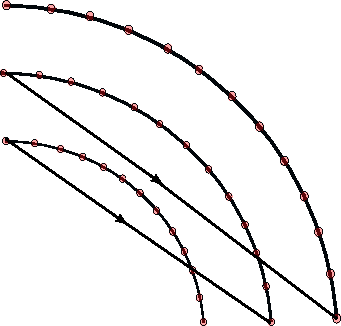
\includegraphics[origin=bl,height=40mm]{./figures/cyclotron/CarbonFieldFormat.pdf}
    \caption{2D field map on the median plane with primary direction corresponding to the azimuthal direction, secondary direction to the radial direction}
    \label{fig:CYCLField}
  \end{center}
\end{figure}
We need to add 6 parameters at the header of a plain $B_z$ [\si{\kilo\gauss}] data file, namely,
$r_{min}$ [\si{\milli\meter}], $\Delta r$ [\si{\milli\meter}], $\theta_{min}$ [\si{\degree}], $\Delta \theta$ [\si{\degree}],
$N_\theta$ (total data number in each arc path of azimuthal direction) and $N_r$ (total path number along radial direction).
If $\Delta r$ or $\Delta \theta$ is decimal, one can set its negative opposite number. For instance, if $\Delta \theta = \frac{1}{3}\si{\degree}$, the fourth line of the header should be set to -3.0.
Example showing the above explained format:
\begin{example}
3.0e+03
10.0
0.0
-3.0
300
161
1.414e-03  3.743e-03  8.517e-03  1.221e-02  2.296e-02
3.884e-02  5.999e-02  8.580e-02  1.150e-01  1.461e-01
1.779e-01  2.090e-01  2.392e-01  2.682e-01  2.964e-01
3.245e-01  3.534e-01  3.843e-01  4.184e-01  4.573e-01
                        ......
\end{example}

\subsection{CYCIAE type}

If \keyword{TYPE=CYCIAE}, the program requires data format given by ANSYS\,10.0.  This function is originally for the \SI{100}{\mega\electronvolt} cyclotron of CIAE,
 whose isochronous fields is numerically computed by by ANSYS. The median plane fields data is output by reading the APDL (ANSYS Parametric Design Language) script
during the post-processing phase (you may need to do minor changes to adapt your own cyclotron model):

\begin{example}
/post1
resume,solu,db
csys,1
nsel,s,loc,x,0
nsel,r,loc,y,0
nsel,r,loc,z,0
PRNSOL,B,COMP

CSYS,1
rsys,1

*do,count,0,200
   path,cyc100_Ansys,2,5,45
   ppath,1,,0.01*count,0,,1
   ppath,2,,0.01*count/sqrt(2),0.01*count/sqrt(2),,1

   pdef,bz,b,z
   paget,data,table

   *if,count,eq,0,then
      /output,cyc100_ANSYS,dat
      *STATUS,data,,,5,5
      /output
   *else
      /output,cyc100_ANSYS,dat,,append
      *STATUS,data,,,5,5
      /output
   *endif
*enddo
finish
\end{example}

By running this in ANSYS, you can get a fields file with the name \filename{cyc100\_ANSYS.data}.
You need to  put 6 parameters at the header of the file, namely,
$r_{min}$ [\si{\milli\meter}], $\Delta r$ [\si{\milli\meter}], $\theta_{min}$[\si{\degree}], $\Delta \theta$[\si{\degree}],
$N_\theta$(total data number in each arc path of azimuthal direction) and $N_r$(total path number along radial direction).
If $\Delta r$ or $\Delta \theta$ is decimal,one can set its negative opposite number. This is useful is the decimal is unlimited.
For instance,if $\Delta \theta = \frac{1}{3} \si{\degree}$, the fourth line of the header should be -3.0.
In a word, the fields are stored in the following format:

\begin{example}
0.0
10.0
0.0e+00
1.0e+00
90
201
 PARAMETER STATUS- DATA  ( 336 PARAMETERS DEFINED)
                  (INCLUDING    17 INTERNAL PARAMETERS)

      LOCATION                VALUE
        1       5       1   0.537657876
        2       5       1   0.538079473
        3       5       1   0.539086731
                  ......
       44       5       1   0.760777286
       45       5       1   0.760918663
       46       5       1   0.760969074

 PARAMETER STATUS- DATA  ( 336 PARAMETERS DEFINED)
                  (INCLUDING    17 INTERNAL PARAMETERS)

      LOCATION                VALUE
        1       5       1   0.704927299
        2       5       1   0.705050993
        3       5       1   0.705341275
                  ......
\end{example}

\subsection{BANDRF type}
If \keyword{TYPE=BANDRF},  the program requires the $B_z$ data format which is same as \keyword{CARBONCYCL}.
But with \keyword{BANDRF} type, the program can also read in the 3D electric field(s).
For the detail about its usage, please see \secref{cyclotron}.

\subsection{Default PSI format}
If the value of \keyword{TYPE} is other string rather than above mentioned, the program requires the data format like  PSI format field file \filename{ZYKL9Z.NAR} and \filename{SO3AV.NAR}, which was given by the measurement.
We add 4 parameters at the header of the file, namely,
$r_{min}$ [\si{\milli\meter}], $\Delta r$ [\si{\milli\meter}], $\theta_{min}$[\si{\degree}], $\Delta \theta$[\si{\degree}],
If $\Delta r$ or $\Delta \theta$ is decimal,one can set its negative opposite number. This is useful is the decimal is unlimited.
For instance,if $\Delta \theta = \frac{1}{3}\si{\degree}$, the fourth line of the header should be -3.0.

\begin{example}
1900.0
20.0
0.0
-3.0
 LABEL=S03AV
 CFELD=FIELD     NREC=  141      NPAR=    3
 LPAR=    7      IENT=    1      IPAR=    1
               3             141             135              30               8
               8              70
 LPAR= 1089      IENT=    2      IPAR=    2
 0.100000000E+01 0.190000000E+04 0.200000000E+02 0.000000000E+00 0.333333343E+00
 0.506500015E+02 0.600000000E+01 0.938255981E+03 0.100000000E+01 0.240956593E+01
 0.282477260E+01 0.340503168E+01 0.419502926E+01 0.505867147E+01 0.550443363E+01
 0.570645094E+01 0.579413509E+01 0.583940887E+01 0.586580372E+01 0.588523722E+01
                        ......
\end{example}

\subsection{3D field-map}

% NOTE: \keyword{SBEND3D}, \keyword{RINGDEFINITION} in elements.tex and \ubsection {3D fieldmap} in
% opalcycl.tex all refer to each other - if updating one check for update on
% others to keep them consistent.

It is additionally possible to load 3D field-maps for tracking through \opalcycl.
3D field-maps are loaded by sequentially adding new field elements to a line,
as is done in \opalt. It is not possible to add
RF cavities while operating in this mode. In order to define ring parameters
such as initial ring radius a \keyword{RINGDEFINITION} type is loaded into the line,
followed by one or more \keyword{SBEND3D} elements.

\begin{example}
ringdef: RINGDEFINITION, HARMONIC_NUMBER=6, LAT_RINIT=2350.0, LAT_PHIINIT=0.0,
         LAT_THETAINIT=0.0, BEAM_PHIINIT=0.0, BEAM_PRINIT=0.0,
         BEAM_RINIT=2266.0, SYMMETRY=4.0, RFFREQ=0.2;

triplet: SBEND3D, FMAPFN="fdf-tosca-field-map.table", LENGTH_UNITS=10., FIELD_UNITS=-1e-4;

l1: Line = (ringdef, triplet, triplet);
\end{example}

The field-map with file name \filename{fdf-tosca-field-map.table} is loaded, which is a
file like
\begin{example}
      422280      422280      422280           1
 1 X [LENGU]
 2 Y [LENGU]
 3 Z [LENGU]
 4 BX [FLUXU]
 5 BY [FLUXU]
 6 BZ [FLUXU]
 0
 194.01470 0.0000000 80.363520 0.68275932346E-07 -5.3752492577 0.28280706805E-07
 194.36351 0.0000000 79.516210 0.42525693524E-07 -5.3827955117 0.17681348191E-07
 194.70861 0.0000000 78.667380 0.19766168358E-07 -5.4350026348 0.82540823165E-08
<continues>
\end{example}
The header parameters are ignored - user supplied parameters \keyword{LENGTH\_UNITS}
and \keyword{FIELD\_UNITS} are used. Fields are supplied on points in a grid in
$(r, y, \phi)$. Positions and field elements are specified by Cartesian
coordinates $(x, y, z)$.

\subsection{User's own field-map}

{ You should revise the function or write your own function according to the instructions in the code to match your own field
format if it is different to above types.}
For more detail about the parameters of \keyword{CYCLOTRON}, please refer to \secref{cyclotron}.

% -- -- -- -- -- -- Section -- -- -- -- -- --
\section{RF field}
\label{sec:opalcycl:rffieldmap}
\subsection{Read RF voltage profile}
The RF cavities are treated as straight lines with infinitely narrow gaps
and the electric field is a $\delta$ function plus a transit time correction.
the two-gap cavity is treated as two independent single-gap cavities. the spiral gap cavity is not implemented yet.
For more detail about the parameters of cyclotron cavities, see \secref{cavity-cycl}.

The voltage profile of a cavity gap  is read from ASCII file. Here is an example:
\begin{example}
6
0.00      0.15      2.40
0.20      0.65      2.41
0.40      0.98      0.66
0.60      0.88     -1.59
0.80      0.43     -2.65
1.00     -0.05     -1.71
\end{example}
The number in the first line means 6 sample points and in the following lines the three values represent the normalized distance to
the inner edge of the cavity, the normalized voltage and its derivative respectively.

\subsection{Read 3D RF field-map}
The 3D RF field-map can be read from H5hut type file. This is useful for modeling the central region electric fields which usually has complicate shapes. For the detail about its usage, please see \secref{cyclotron}.

Please note that in this case, the E field is treated as a part of \keyword{CYCLOTRON} element, rather than a independent \keyword{RFCAVITY} element.
% -- -- -- -- -- -- Section -- -- -- -- -- --
\section{Particle Tracking and Acceleration}

The precision of the tracking methods is vital for the entire simulation process, especially for long distance tracking jobs.
\opalcycl uses a \engordnumber{4} order Runge-Kutta algorithm and the \engordnumber{2} order Leap-Frog scheme. The \engordnumber{4} order Runge-Kutta algorithm needs four external magnetic field evaluation in each time step $\tau$ .
During the field interpolation process, for an arbitrary given point the code first interpolates Formula $B_z$
for its counterpart on the median plane and then expands to this give point using \eqnref{Bfield}.

After each time step $i$, the code detects whether the particle crosses any one of the RF cavities during this step.
If it does, the time point $t_c$ of crossing is calculated and the particle return back to the start point of
step $i$. Then this step is divided into three sub-steps:
first, the code tracks this particle for $ t_1 = \tau - (t_c-t_{i-1})$;
then it calculates the voltage and adds momentum kick to the particle and refreshes its relativistic parameters $\beta$ and $\gamma$;
and then tracks it for $t_2 = \tau - t_1$.

% -- -- -- -- -- -- Section -- -- -- -- -- --
\section{Space Charge}

\opalcycl uses the same solvers as \opalt to calculate the space charge effects \seechp{fieldsolver}.

Typically, the space charge field is calculated once per time step. This is no surprise for the \engordnumber{2} order Boris-Buneman time integrator (leapfrog-like scheme) which has per default only one force evaluation per step. The \engordnumber{4} order Runge-Kutta integrator keeps the space charge field constant for one step, although there are four external field evaluations. There is an experimental multiple-time-stepping (MTS) variant of the Boris-Buneman/leapfrog-method, which evaluates space charge only every N\engordletters{th} step, thus greatly reducing computation time while usually being still accurate enough.


% -- -- -- -- -- -- Section -- -- -- -- -- --
\section{Multi-bunch Mode}
\label{sec:opalcycl:MultiBunch}

The neighboring bunches problem is motivated by the fact that for high intensity cyclotrons with small turn
separation, single bunch space charge effects are not the only contribution. Along with the increment of beam
current, the mutual interaction of neighboring bunches in radial direction becomes more and more important,
especially at large radius where the distances between neighboring bunches get increasingly small and even they
can overlap each other. One good example is PSI \SI{590}{\mega\electronvolt} Ring cyclotron with a current of about \SI{2}{\milli\ampere} in
CW operation and the beam power amounts to \SI{1.2}{\mega\watt}. An upgrade project for Ring is in process with
the goal of \SI{1.8}{\mega\watt} CW on target by replacing four old aluminum resonators by four new copper cavities with peak
voltage increasing from about \SI{0.7}{\mega\watt} to above \SI{0.9}{\mega\watt}. After upgrade, the total turn
number is reduced from 200 turns to less then 170 turns.
Turn separation is increased a little bit, but still are at the same order
of magnitude as the radial size of the bunches. Hence once the beam current increases from \SI{2}{\milli\ampere} to \SI{3}{\milli\ampere}, the mutual space
charge effects between radially neighboring bunches can have significant impact on beam dynamics.
In consequence, it is important to cover neighboring bunch effects in the simulation to quantitatively study its impact on the beam dynamics.

In \opalcycl, we developed a new fully consistent algorithm of multi-bunch simulation.  We implemented two working modes, namely ,
\keyword{AUTO} and \keyword{FORCE}. In the first mode, only a single bunch is tracked and accelerated at the beginning,
until the radial neighboring bunch effects become an important factor to the bunches' behavior. Then the new bunches will be injected automatically to take these effects into account. In this way, we can save time and memory, and more important,
we can get higher precision for the simulation in the region where neighboring bunch effects are important.
In the other mode, multi-bunch simulation starts from the injection points.

In the space charge calculation for multi-bunch, the computation region covers all bunches.
Because the energy of the bunches is quite different, it is inappropriate to use only one particle rest frame and a single Lorentz transformation any more.
So the particles are grouped into different energy bins and in each bin the energy spread is relatively small. We apply Lorentz transforming, calculate
the space charge fields and apply the back Lorentz transforming for each bin separately. Then add the field data together. Each particle has a ID number to identify
which energy bin it belongs to.


% -- -- -- -- -- -- Section -- -- -- -- -- --
\section{Input}
All the three working modes of \opalcycl use an input file written in \mad language which will be described in detail in the following chapters.

For the  {\bfseries Tune Calculation mode}, one additional auxiliary file with the following format is needed.
\begin{example}
   72.000 2131.4   -0.240
   74.000 2155.1   -0.296
   76.000 2179.7   -0.319
   78.000 2204.7   -0.309
   80.000 2229.6   -0.264
   82.000 2254.0   -0.166
   84.000 2278.0    0.025
\end{example}
In each line the three values represent energy $E$, radius $r$ and $P_r$ for the SEO (Static Equilibrium Orbit)
at starting point respectively and their units are \si{\mega\electronvolt}, \si{\milli\meter} and \si{\milli\radian}.

A bash script \filename{tuning.sh} is shown on the next page, to execute \opalcycl for tune calculations.
\examplefromfile{examples/tuning.sh}
To start execution, just run \filename{tuning.sh} which uses the input file \filename{testcycl.in} and the auxiliary file \filename{FIXPO\_ SEO}.
The output file is \filename{plotdata} from which one can plot the tune diagram.


% -- -- -- -- -- -- Section -- -- -- -- -- --
\section{Output}
\subsubsection{Single Particle Tracking mode}

The intermediate phase space data is stored in an ASCII file which can be used to
the plot the orbit. The file's name is combined by input file name (without extension) and \filename{-trackOrbit.dat}.
The data are stored in the global Cartesian coordinates.
The frequency of the data output can be set using the  option \keyword{SPTDUMPFREQ} of \keyword{OPTION} statement \seesec{option}

The phase space data per \keyword{STEPSPERTURN} (a parameter in the \keyword{TRACK} command) steps is stored in an ASCII file.
The file's name is a combination of input file name (without extension) and \filename{-afterEachTurn.dat}.
The data is stored in the global cylindrical coordinate system.
Please note that if the field map is ideally isochronous, the reference particle of a given energy take exactly one revolution in \keyword{STEPPERTURN} steps;
Otherwise, the particle may not go through a full \SI{360}{\degree} in \keyword{STEPPERTURN} steps.

There are 3 ASCII files which store the phase space data around $0$, $\pi/8$ and $\pi/4$ azimuths.
Their names are the combinations of input file name (without extension) and \filename{-Angle0.dat}, \filename{-Angle1.dat} and \filename{-Angle2.dat} respectively.
The data is stored in the global cylindrical coordinate system, which can be used to check the property of the closed orbit.

\subsubsection{Tune calculation mode}

 The tunes $\nu_r$ and $\nu_z$ of each energy are stored in a ASCII file with name \filename{tuningresult}.

\subsubsection{Multi-particle tracking mode}

The intermediate phase space data of all particles and some interesting parameters,
including RMS envelop size, RMS emittance, external field, time, energy, length of path, number of bunches and
tracking step, are stored in the H5hut file-format \cite{bib:howison2010} and can be analyzed
using the H5root \cite{bib:schietinger}.
The frequency of the data output can be set using the  \keyword{PSDUMPFREQ} option of \keyword{OPTION} statement \seesec{option}.
The file is named like the input file but the extension is \filename{.h5}.

The intermediate phase space data of central particle (with ID of 0) and an off-centering particle (with ID of 1)
are stored in an ASCII file. The file's name is combined by the input file name (without extension) and \filename{-trackOrbit.dat}.
The frequency of the data output can be set using the \keyword{SPTDUMPFREQ} option of \keyword{OPTION} statement \seesec{option}.



\section{Matched Distribution}
In order to run matched distribution simulation one has to specify a periodic accelerator. The function call also needs
the symmetry of the machine as well as a field map. The user then specifies the emittance $\pi\si{\milli\meter\milli\radian}$.
\begin{verbatim}
/*
 * specify periodic accelerator
 */
l1 = ...

/*
 * try finding a matched distribution
 */
Dist1:DISTRIBUTION, TYPE=GAUSSMATCHED, LINE=l1, FMAPFN=...,
                    MAGSYM=..., EX = ..., EY = ..., ET = ...;
\end{verbatim}
\subsection{Example}
Simulation of the PSI Ring Cyclotron at \SI{580}{\mega\electronvolt} and current \SI{2.2}{\milli\ampere}. The program finds a matched
distribution followed by a bunch initialization according to the matched covariance matrix.\\
The matched distribution algorithm works with normalized emittances, i.e. normalized by the lowest energy of the
machine. The printed emittances, however, are the geometric emittances. In addition, it has to
be paid attention that the computation is based on $(x,x',y,y',z,\delta)$ instead of $(x,p_{x},y,p_{y},z,p_{z})$. Since
the particles are represented in the latter coordinate system, the corresponding transformation has to be applied to
obtain the rms emittances that are given in the output.
\subsubsection{Input file}
\examplefromfile{examples/matchedDistribution.in}
\subsubsection{Output}
\examplefromfile{examples/matchedDistribution.output}

%----------- Footer control ------------------
\ifthenelse{\boolean{FullOPALManual}}
{
  %do nothing
}
% else (for individual document creation)
{
\appendix
\printbibliography
\end{document}
}
%---------------------------------------------
